\documentclass{article}\usepackage[]{graphicx}\usepackage[]{color}
%% maxwidth is the original width if it is less than linewidth
%% otherwise use linewidth (to make sure the graphics do not exceed the margin)
\makeatletter
\def\maxwidth{ %
  \ifdim\Gin@nat@width>\linewidth
    \linewidth
  \else
    \Gin@nat@width
  \fi
}
\makeatother

\definecolor{fgcolor}{rgb}{0.345, 0.345, 0.345}
\newcommand{\hlnum}[1]{\textcolor[rgb]{0.686,0.059,0.569}{#1}}%
\newcommand{\hlstr}[1]{\textcolor[rgb]{0.192,0.494,0.8}{#1}}%
\newcommand{\hlcom}[1]{\textcolor[rgb]{0.678,0.584,0.686}{\textit{#1}}}%
\newcommand{\hlopt}[1]{\textcolor[rgb]{0,0,0}{#1}}%
\newcommand{\hlstd}[1]{\textcolor[rgb]{0.345,0.345,0.345}{#1}}%
\newcommand{\hlkwa}[1]{\textcolor[rgb]{0.161,0.373,0.58}{\textbf{#1}}}%
\newcommand{\hlkwb}[1]{\textcolor[rgb]{0.69,0.353,0.396}{#1}}%
\newcommand{\hlkwc}[1]{\textcolor[rgb]{0.333,0.667,0.333}{#1}}%
\newcommand{\hlkwd}[1]{\textcolor[rgb]{0.737,0.353,0.396}{\textbf{#1}}}%
\let\hlipl\hlkwb

\usepackage{framed}
\makeatletter
\newenvironment{kframe}{%
 \def\at@end@of@kframe{}%
 \ifinner\ifhmode%
  \def\at@end@of@kframe{\end{minipage}}%
  \begin{minipage}{\columnwidth}%
 \fi\fi%
 \def\FrameCommand##1{\hskip\@totalleftmargin \hskip-\fboxsep
 \colorbox{shadecolor}{##1}\hskip-\fboxsep
     % There is no \\@totalrightmargin, so:
     \hskip-\linewidth \hskip-\@totalleftmargin \hskip\columnwidth}%
 \MakeFramed {\advance\hsize-\width
   \@totalleftmargin\z@ \linewidth\hsize
   \@setminipage}}%
 {\par\unskip\endMakeFramed%
 \at@end@of@kframe}
\makeatother

\definecolor{shadecolor}{rgb}{.97, .97, .97}
\definecolor{messagecolor}{rgb}{0, 0, 0}
\definecolor{warningcolor}{rgb}{1, 0, 1}
\definecolor{errorcolor}{rgb}{1, 0, 0}
\newenvironment{knitrout}{}{} % an empty environment to be redefined in TeX

\usepackage{alltt}

 \renewcommand{\familydefault}{\sfdefault}
\IfFileExists{upquote.sty}{\usepackage{upquote}}{}
\begin{document}
\definecolor{blendedblue}{rgb}{0.137,0.466,0.741}

\definecolor{darkred}{rgb}{0.545,0,0}

\begin{knitrout}
\definecolor{shadecolor}{rgb}{0.969, 0.969, 0.969}\color{fgcolor}\begin{kframe}
\begin{alltt}
\hlkwd{set.seed}\hlstd{(}\hlnum{2}\hlstd{)}

\hlstd{OwlRed} \hlkwb{<-} \hlkwd{rgb}\hlstd{(}\hlnum{255}\hlstd{,}  \hlnum{92}\hlstd{,} \hlnum{168}\hlstd{,} \hlkwc{maxColorValue} \hlstd{=} \hlnum{255}\hlstd{)}
\hlstd{OwlGreen} \hlkwb{<-} \hlkwd{rgb}\hlstd{(}\hlnum{90}\hlstd{,} \hlnum{168}\hlstd{,}   \hlnum{0}\hlstd{,} \hlkwc{maxColorValue} \hlstd{=} \hlnum{255}\hlstd{)}
\hlstd{OwlBlue} \hlkwb{<-} \hlkwd{rgb}\hlstd{(} \hlnum{0}\hlstd{,} \hlnum{152}\hlstd{,} \hlnum{233}\hlstd{,} \hlkwc{maxColorValue} \hlstd{=} \hlnum{255}\hlstd{)}
\hlstd{OwlYellow} \hlkwb{<-} \hlkwd{rgb}\hlstd{(} \hlnum{242}\hlstd{,} \hlnum{147}\hlstd{,}  \hlnum{24}\hlstd{,} \hlkwc{maxColorValue} \hlstd{=} \hlnum{255}\hlstd{)}
\end{alltt}
\end{kframe}
\end{knitrout}


\begin{knitrout}
\definecolor{shadecolor}{rgb}{0.969, 0.969, 0.969}\color{fgcolor}

\includegraphics[width=\textwidth]{figure/dice1-1} 


\includegraphics[width=\textwidth]{figure/dice1-2} 

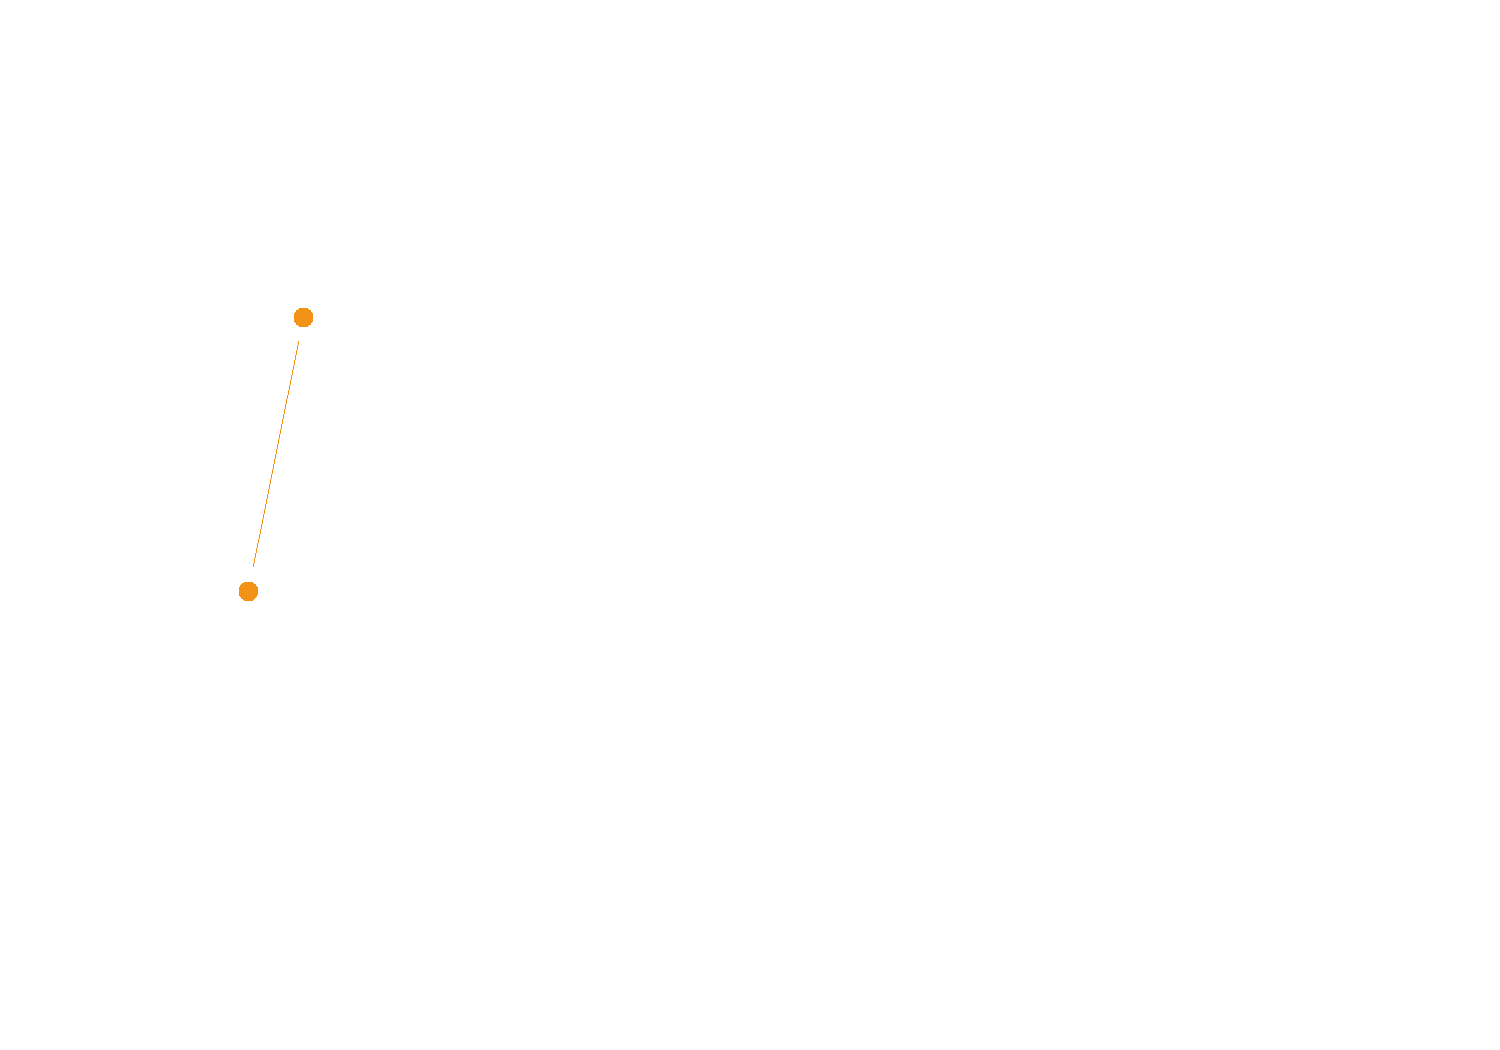
\includegraphics[width=\textwidth]{figure/dice1-3} 

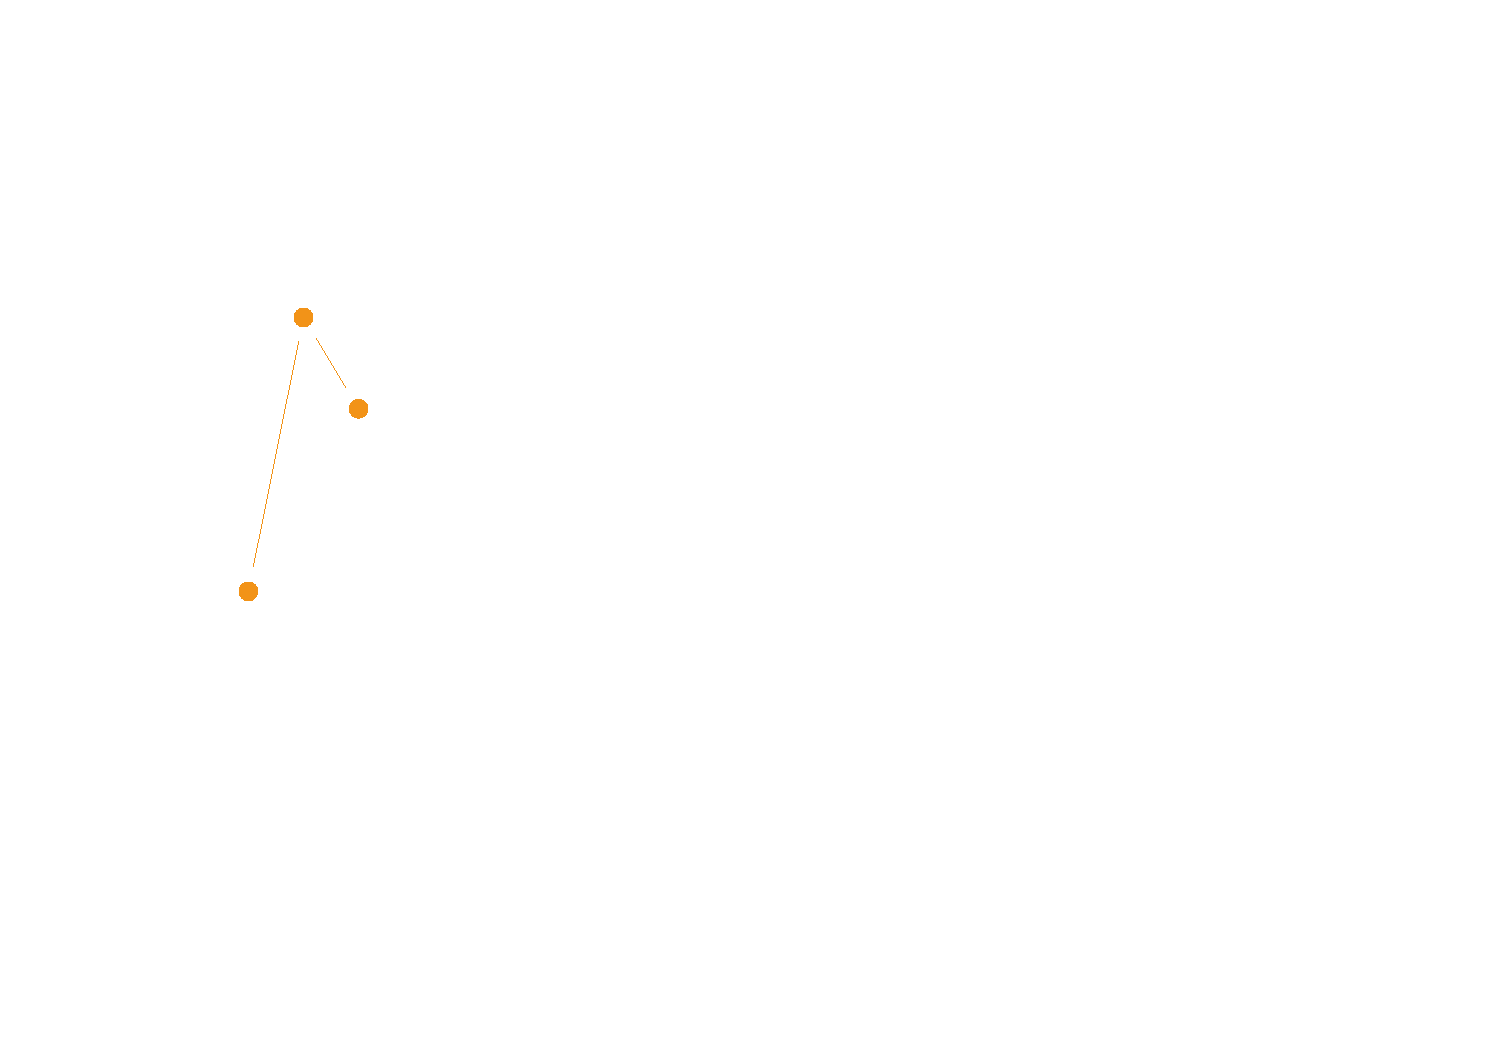
\includegraphics[width=\textwidth]{figure/dice1-4} 

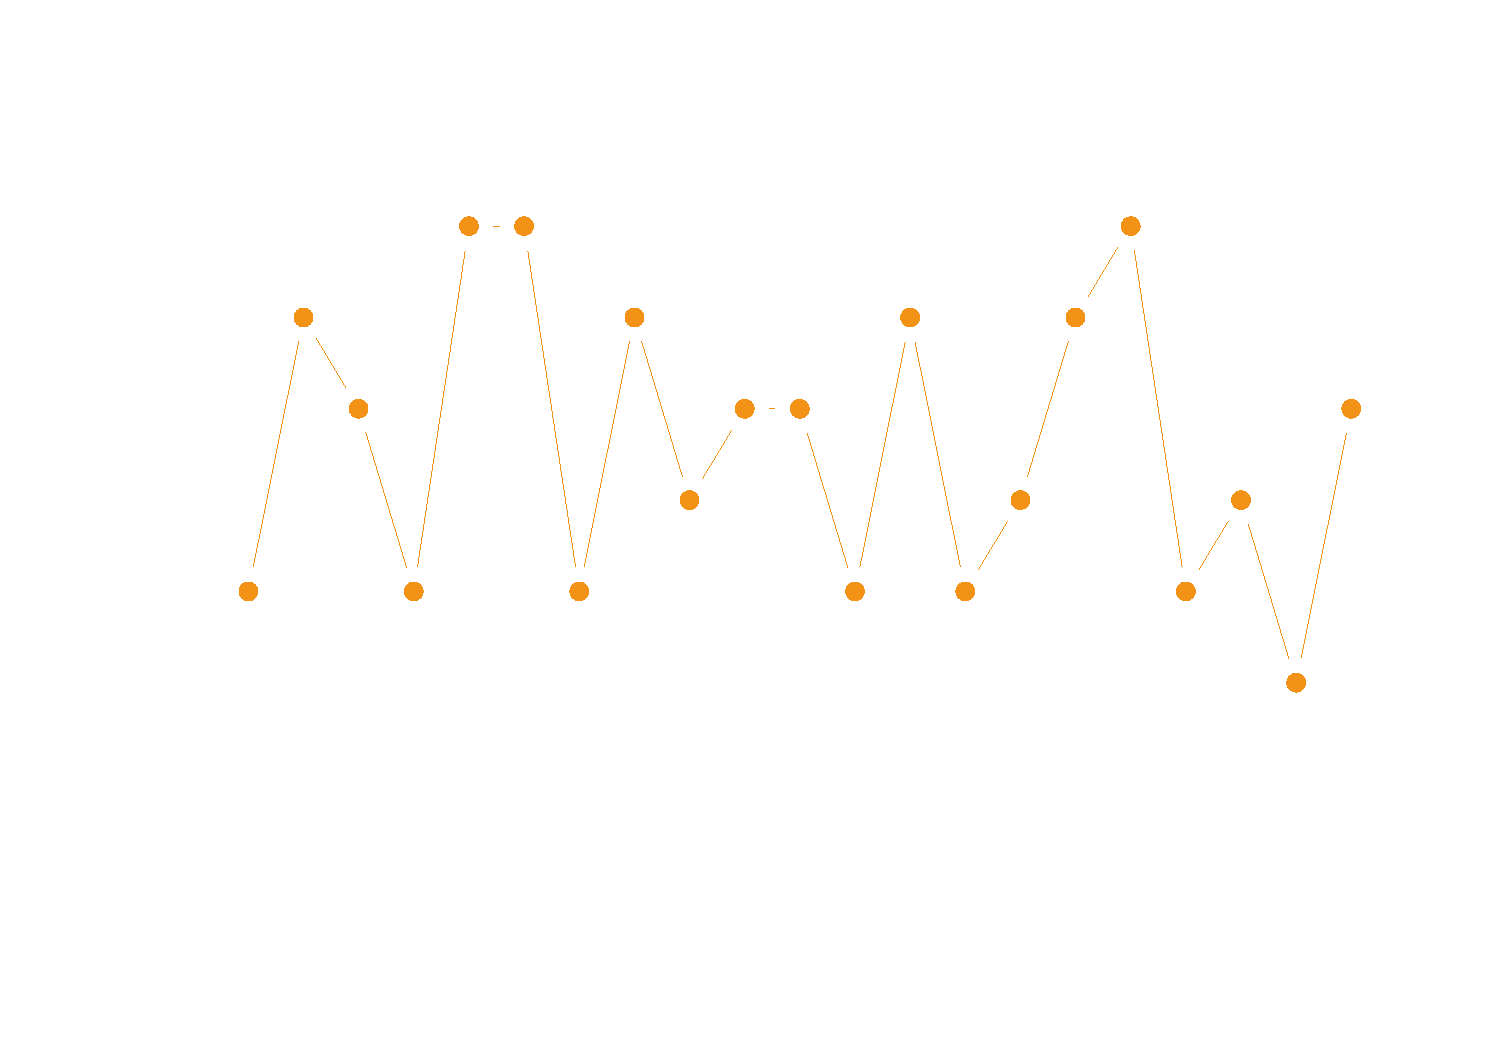
\includegraphics[width=\textwidth]{figure/dice1-5} 

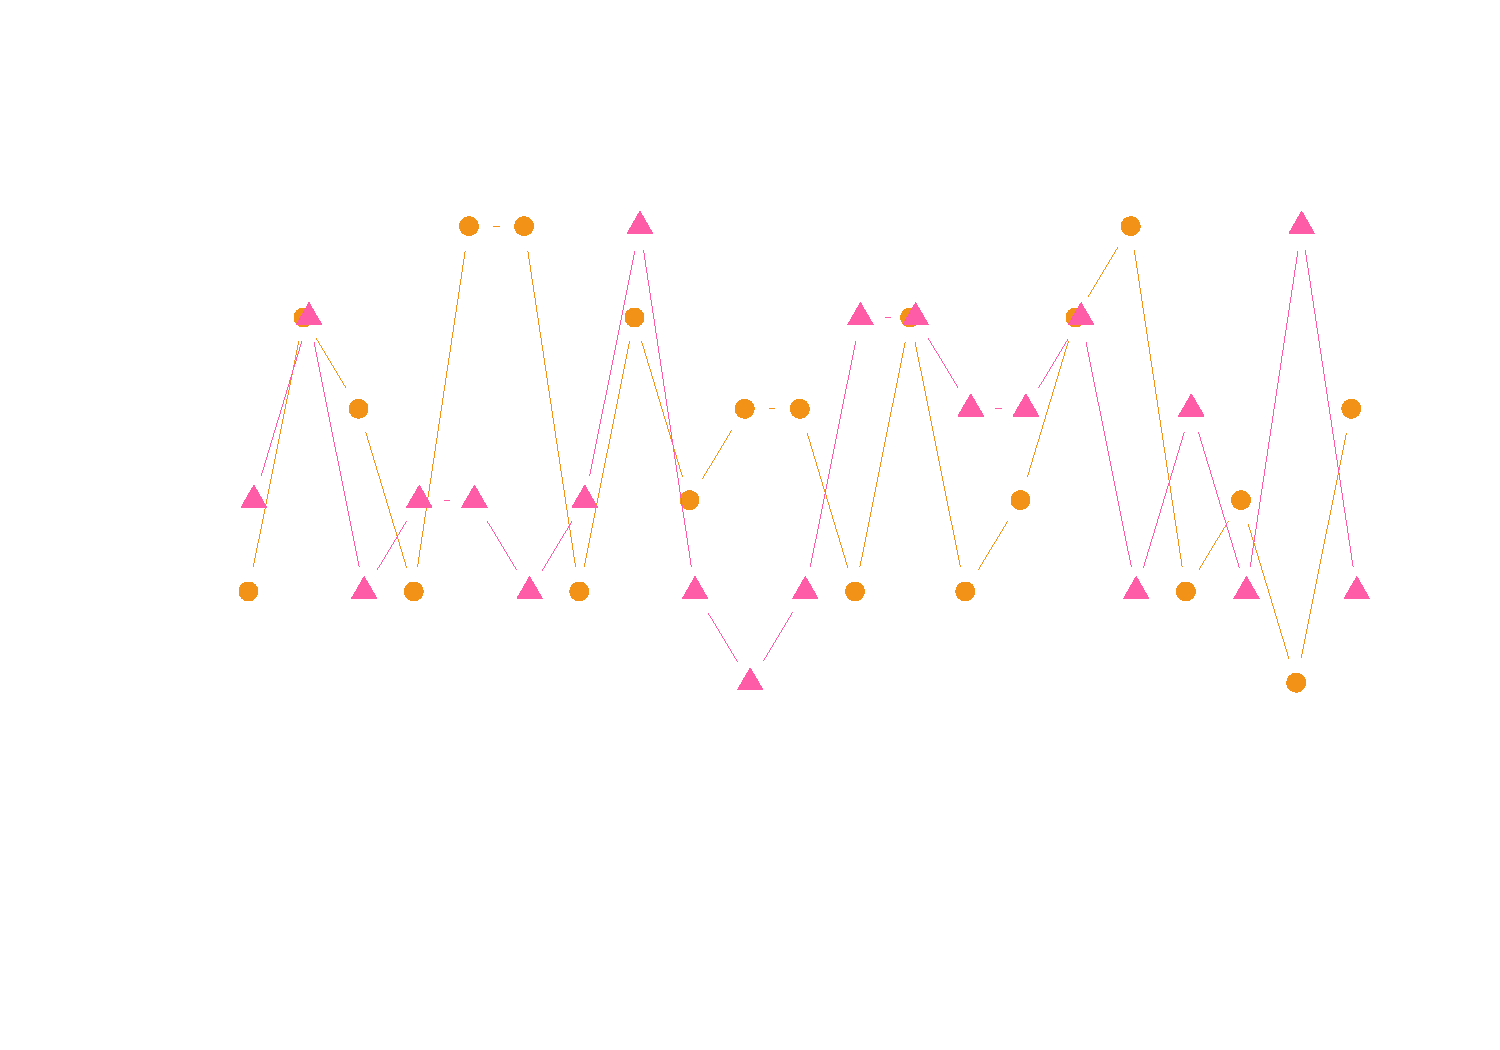
\includegraphics[width=\textwidth]{figure/dice1-6} 

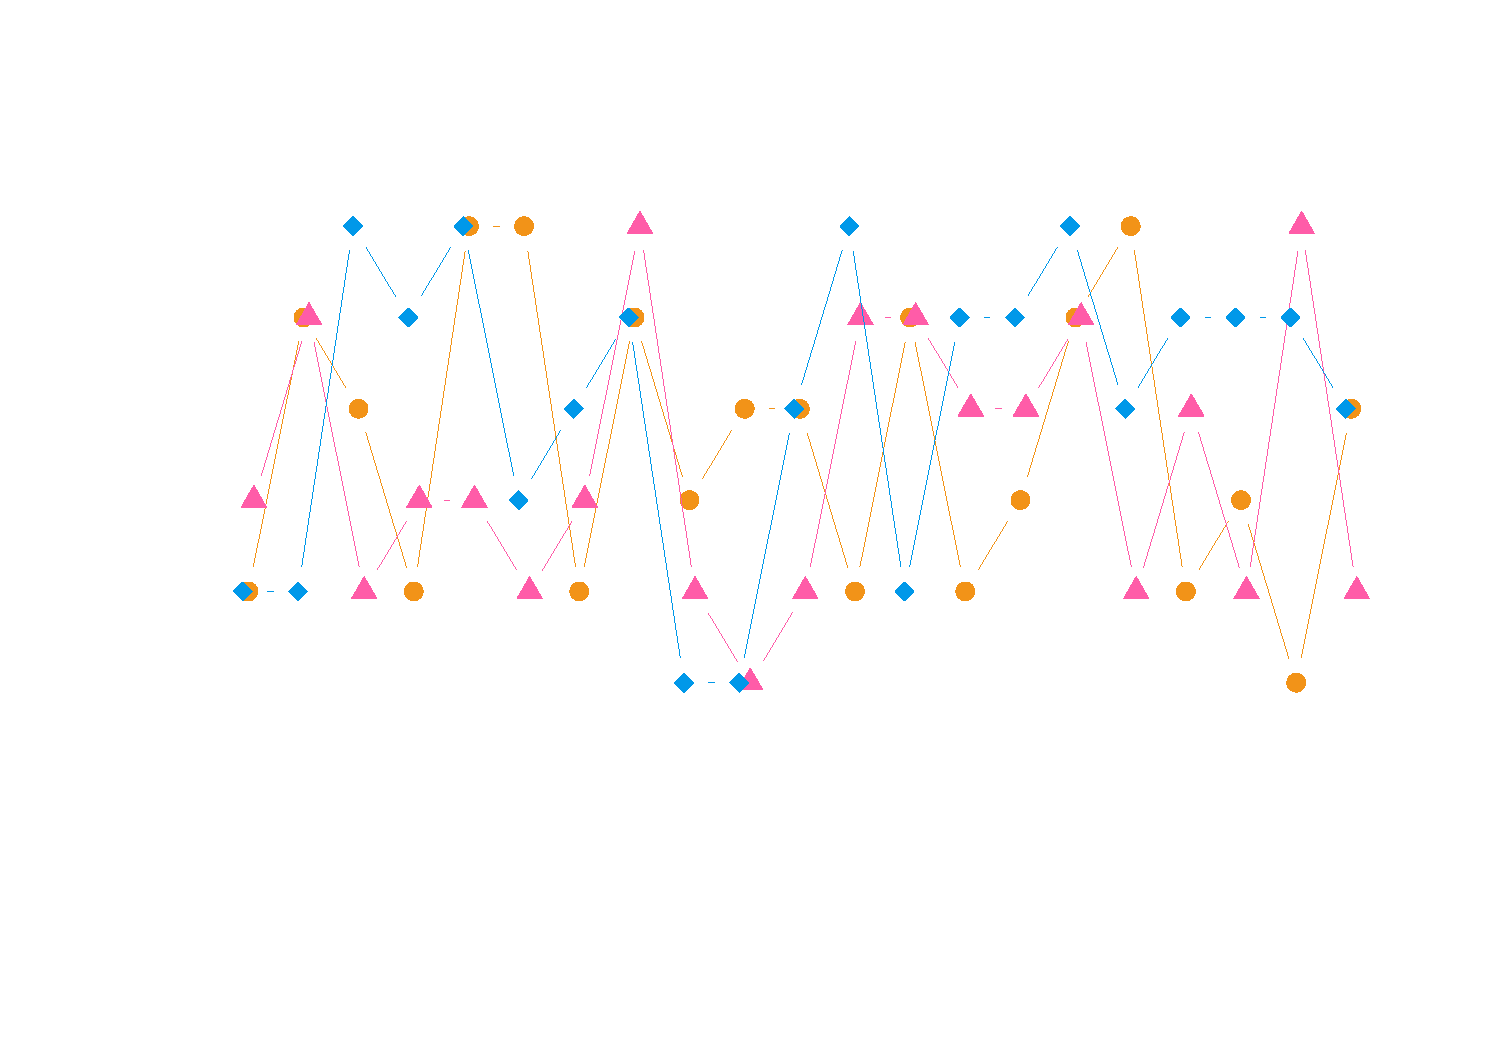
\includegraphics[width=\textwidth]{figure/dice1-7} 

\end{knitrout}


\begin{knitrout}
\definecolor{shadecolor}{rgb}{0.969, 0.969, 0.969}\color{fgcolor}

\includegraphics[width=\textwidth]{figure/dice2-1} 

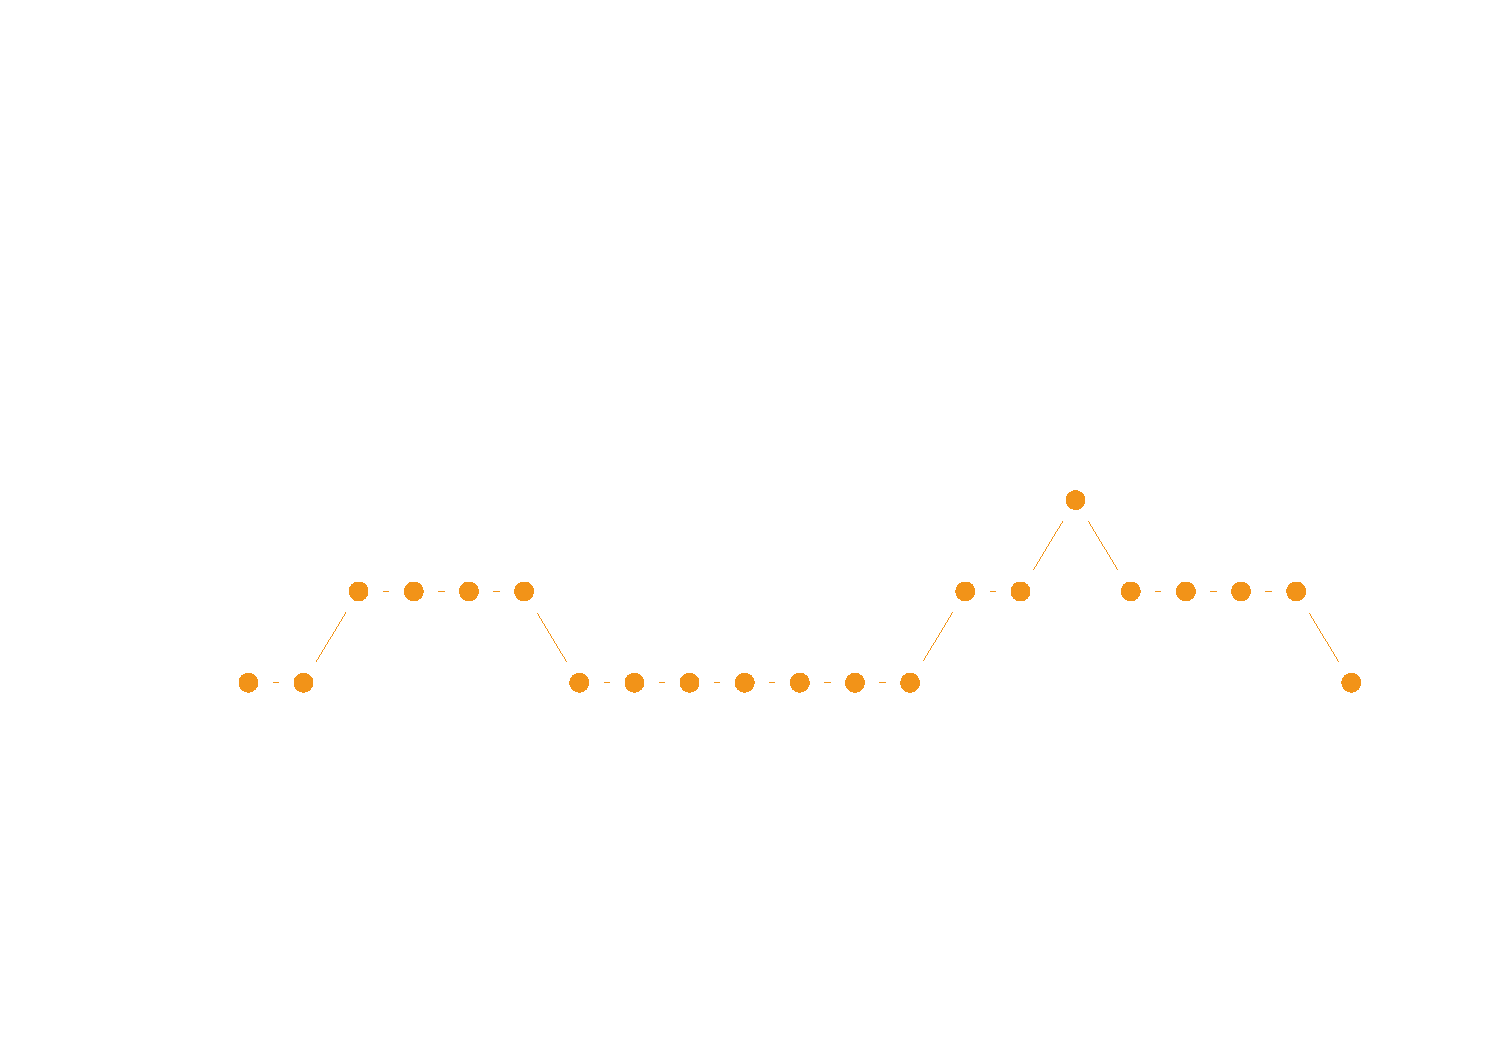
\includegraphics[width=\textwidth]{figure/dice2-2} 

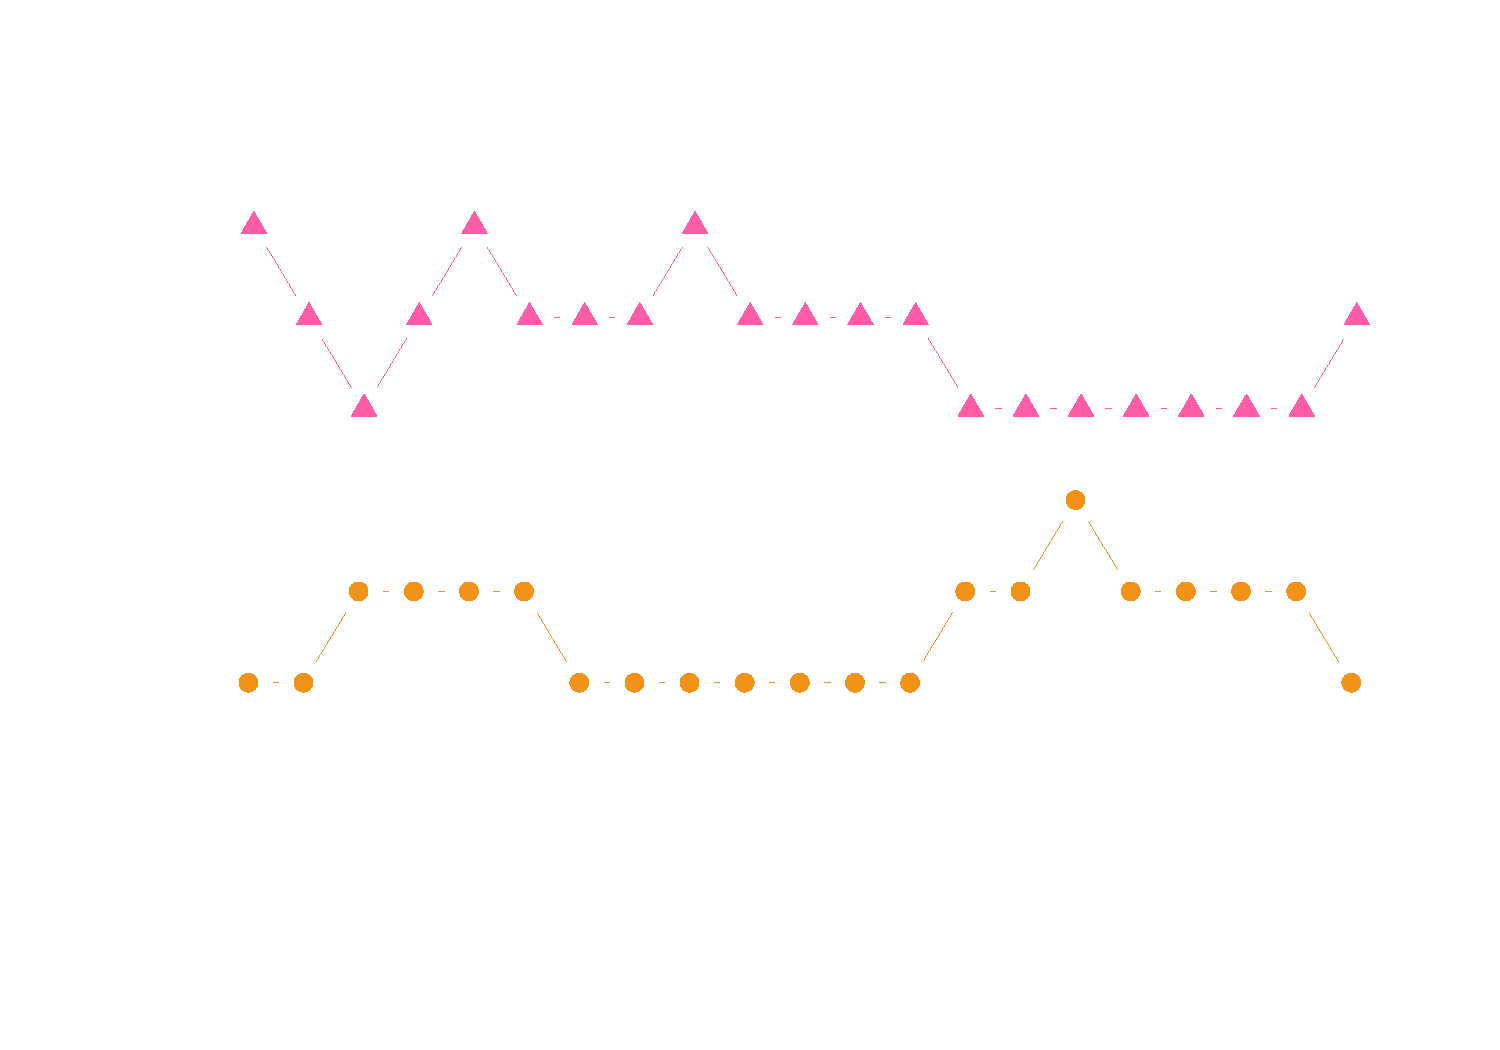
\includegraphics[width=\textwidth]{figure/dice2-3} 

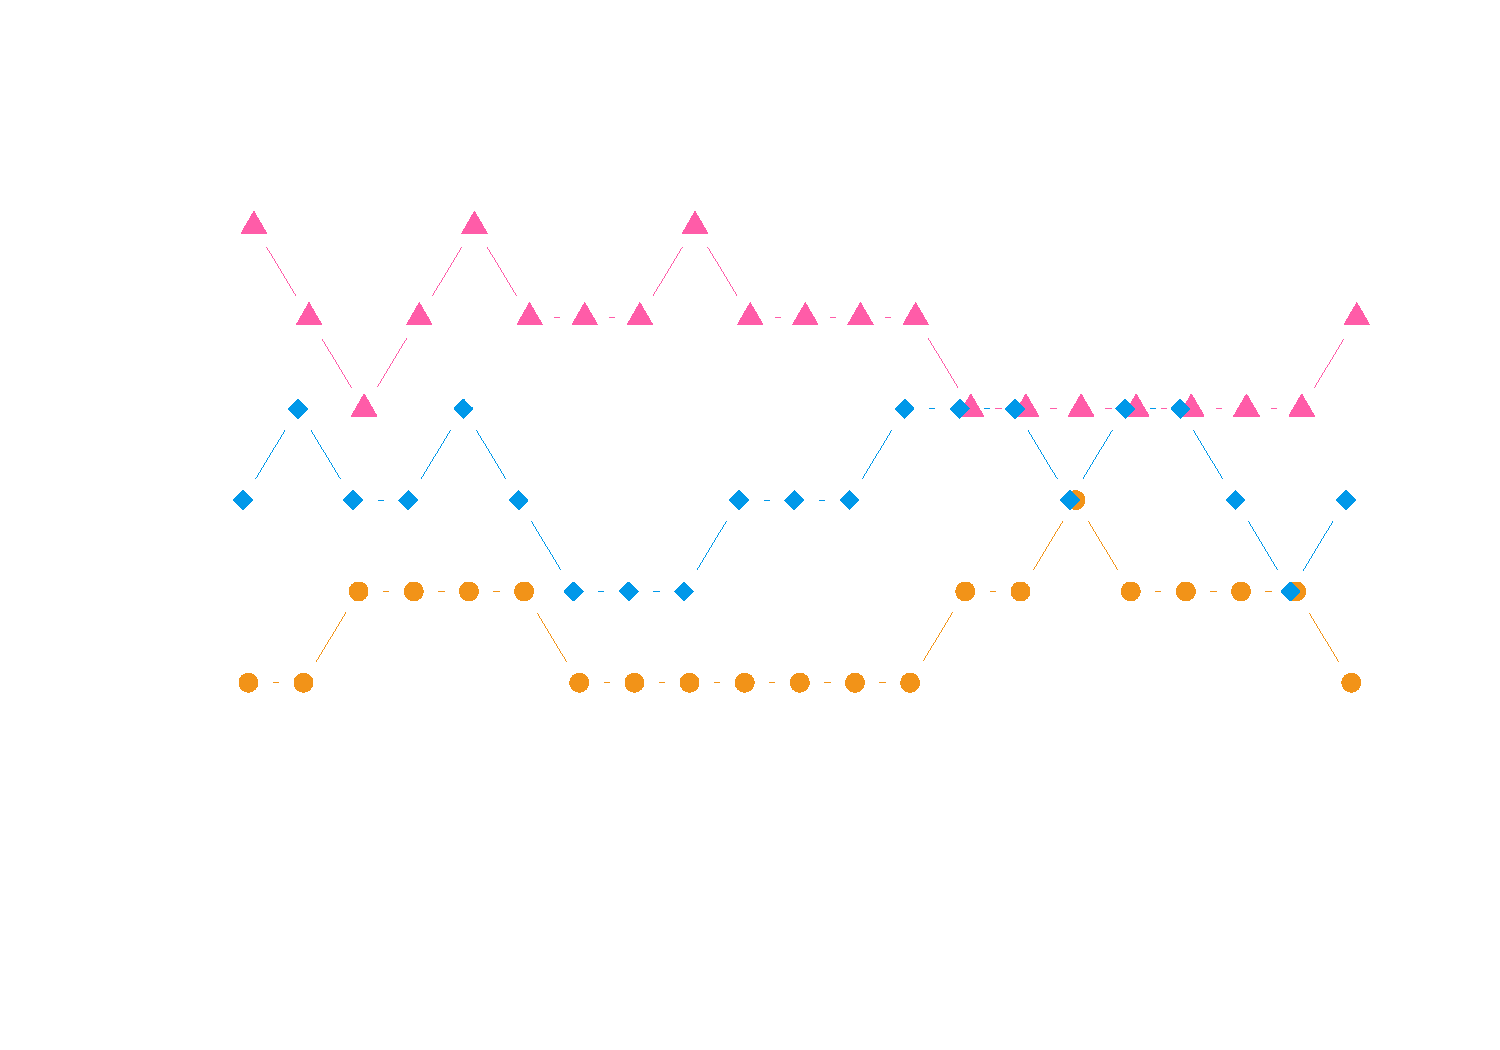
\includegraphics[width=\textwidth]{figure/dice2-4} 

\end{knitrout}

\begin{knitrout}
\definecolor{shadecolor}{rgb}{0.969, 0.969, 0.969}\color{fgcolor}

\includegraphics[width=\textwidth]{figure/resultsdynhet-1} 

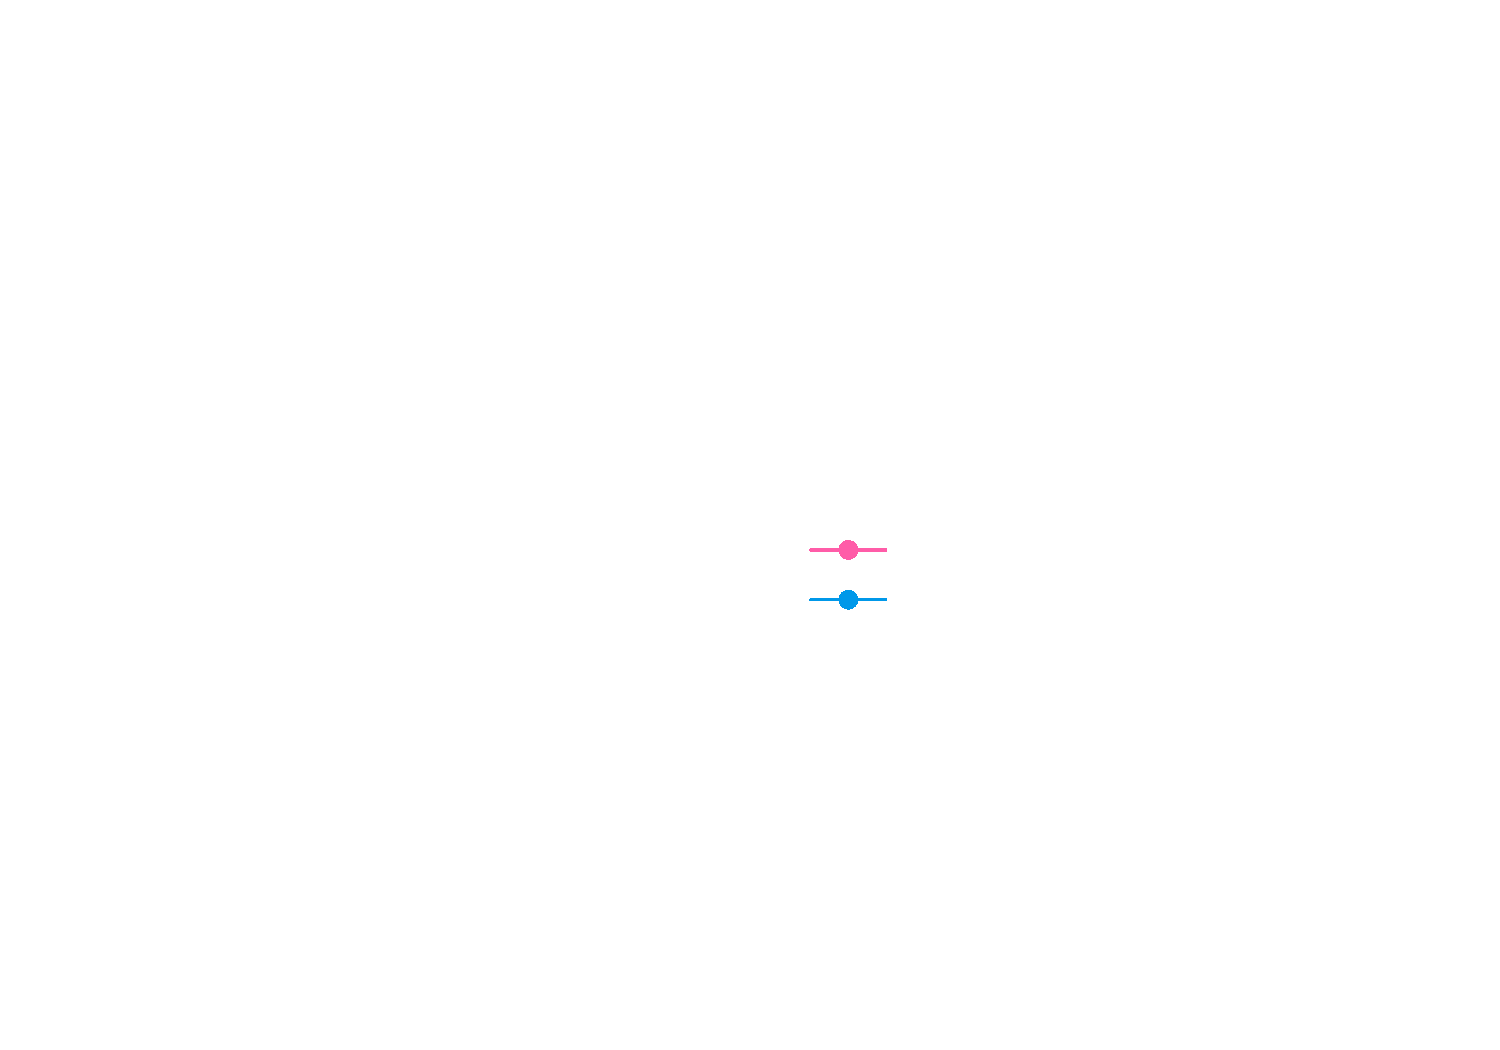
\includegraphics[width=\textwidth]{figure/resultsdynhet-2} 

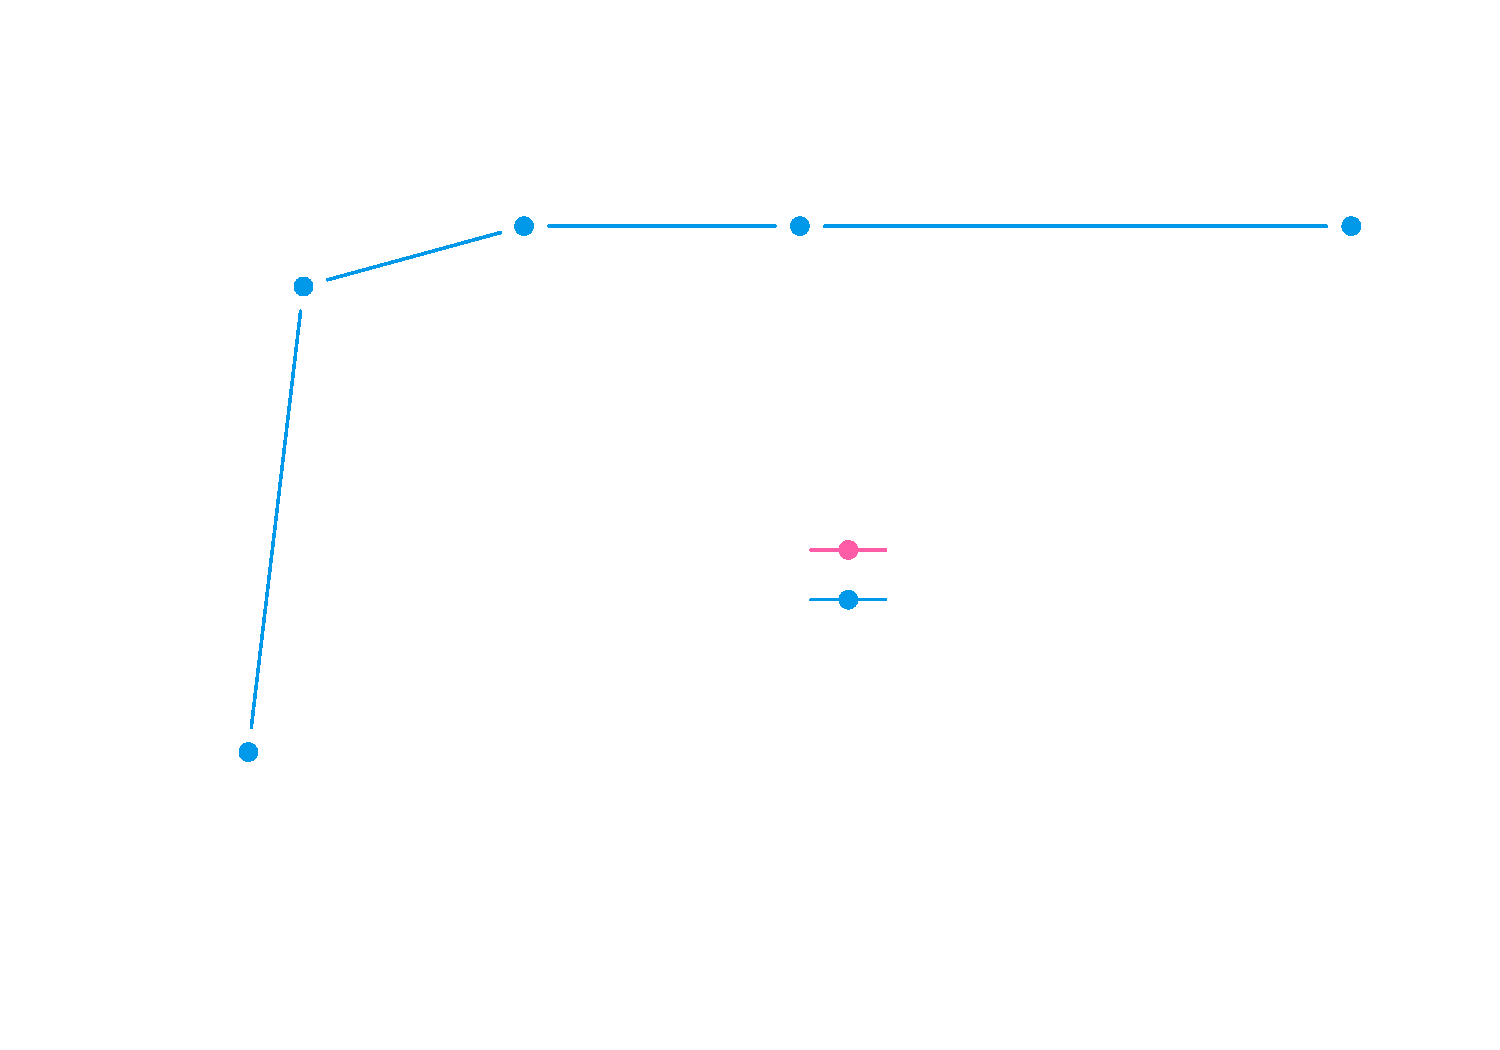
\includegraphics[width=\textwidth]{figure/resultsdynhet-3} 

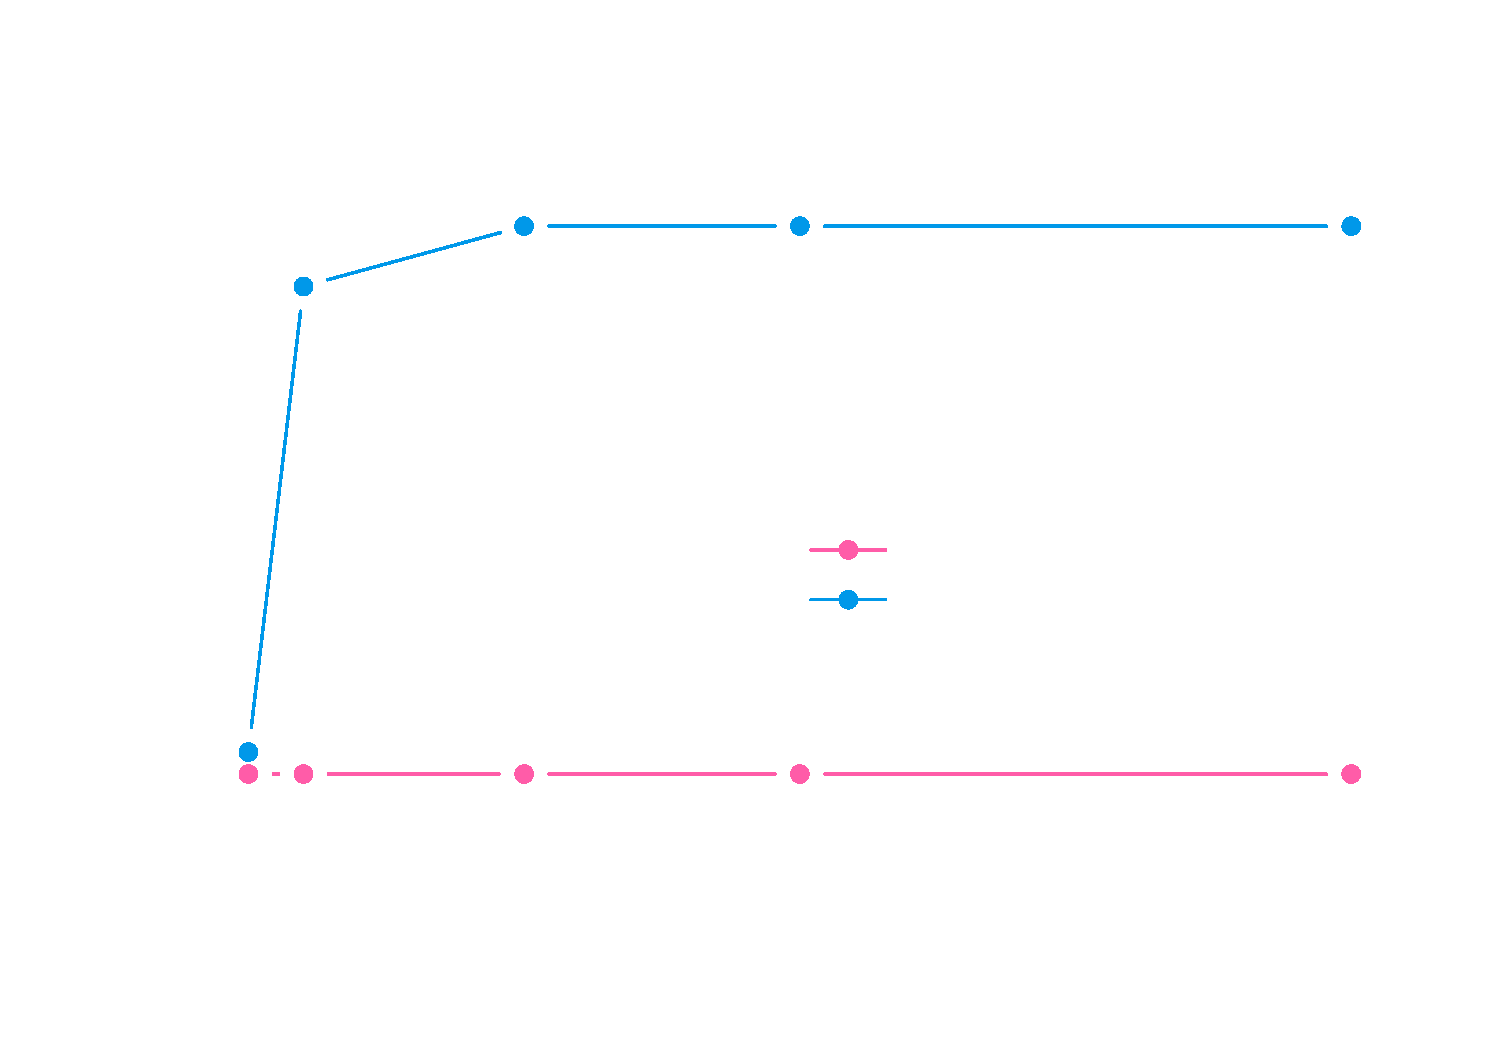
\includegraphics[width=\textwidth]{figure/resultsdynhet-4} 

\end{knitrout}

\end{document}
